% !TEX root = ../main.tex
\section{Zoom covers}\label{app:zoom-covers}

The Local and Exotic components use 38 zoom covers: 30 around the
aligned configurations and eight around the square and pentagon
configurations and the first arc. Each is specified by a small set of
parameters, fixed in the program's source, from which its zooms are built:
the coordinate system (the configuration parameters, or the arc coordinates
\cref{eq:arc-coordinates} of one plane), an invertible affine map to base
and offset coordinates, the boxes $\Sigma$ and $\Phi$, the radii and, for a
point zoom cover, the ratio $\rho_0$. The two tables below list these
parameters; together with the coordinates given in the text, they determine
every cover. The terminal cells and their witnesses are stored in one data
file per cover. Before any search, every cover is rebuilt from its
parameters and checked: the cells of each zoom must tile its domain exactly,
every cell must satisfy the hypotheses of \cref{lem:zoom-lemma}, and every
handed-over cell must satisfy the hypothesis of \cref{lem:hand-over}. The
covered sets are then those of \cref{lem:tube-coverage,lem:point-coverage},
except that the pentagon cover drops the upper bound $\xi\le0$, beyond which
no configuration lies in $D$ (\cref{subsec:eliminating-the-pentagon-configuration}).
The checks take a few seconds; the data files were produced by the
program's generator (\texttt{rid generate}), which is not part of the proof:
every cell is checked exactly before use.

Each Local cover consists of the six face zooms of
\cref{subsec:face-zooms-and-the-local-component} over one viewing rectangle
$W$: its base coordinates are $(s,t)\in W$, its offset is $\mathbf r$ with
$\Phi={[-1,1]}^3$, and its offset radius is $\delta_{\max}$. The rectangles of
\cref{tab:local-covers} have disjoint interiors; each cover's rectangle $W$
is the row enlarged by $1/1024$ on every side and cut to
$W_0=[0,2/3]\times[0,2/5]$, so that neighbouring covers overlap. The rows do
not tile $W_0$: the enlarged rows leave gaps around the square and pentagon
configurations, which those covers fill, and the parts of $W_0$ beyond the
viewing triangle need no cover, since the Domain component eliminates them. \Cref{fig:local-tiling} shows the rows with the square and pentagon covers.
That the covers of aligned configurations together reach every viewing
direction of the triangle is the computation of
\cref{subsec:ranges-and-remaining-touch-configurations}.



\begin{table}[ht]
\centering\small
\begin{tabular}{rllllrr}
  \toprule
  Cover & $s$ from & $s$ to & $t$ from & $t$ to & $\delta_{\max}$ & Cells\\
  \midrule
  0 & $1/12$ & $1/6$ & $0$ & $1/10$ & $1/96$ & 24\\
  1 & $0$ & $1/6$ & $1/10$ & $1/5$ & $1/80$ & 45\\
  2 & $1/6$ & $1/3$ & $0$ & $1/10$ & $1/50$ & 26\\
  3 & $1/6$ & $1/4$ & $1/10$ & $1/5$ & $1/50$ & 27\\
  4 & $1/4$ & $1/3$ & $1/10$ & $3/20$ & $1/50$ & 16\\
  5 & $1/4$ & $1/3$ & $3/20$ & $1/5$ & $1/50$ & 20\\
  6 & $0$ & $1/12$ & $1/5$ & $3/10$ & $1/50$ & 18\\
  7 & $1/12$ & $1/8$ & $1/5$ & $9/40$ & $1/50$ & 27\\
  8 & $1/12$ & $1/8$ & $9/40$ & $1/4$ & $1/50$ & 15\\
  9 & $1/8$ & $1/6$ & $1/5$ & $1/4$ & $1/200$ & 34\\
  10 & $1/12$ & $1/8$ & $1/4$ & $3/10$ & $1/50$ & 15\\
  11 & $1/8$ & $7/48$ & $1/4$ & $11/40$ & $1/50$ & 12\\
  12 & $7/48$ & $1/6$ & $1/4$ & $21/80$ & $1/200$ & 49\\
  13 & $7/48$ & $5/32$ & $21/80$ & $11/40$ & $1/50$ & 12\\
  14 & $5/32$ & $31/192$ & $21/80$ & $43/160$ & $1/200$ & 45\\
  15 & $1/8$ & $1/6$ & $11/40$ & $3/10$ & $1/50$ & 15\\
  16 & $0$ & $1/6$ & $3/10$ & $2/5$ & $1/50$ & 39\\
  17 & $1/6$ & $5/24$ & $1/5$ & $9/40$ & $1/50$ & 22\\
  18 & $1/6$ & $3/16$ & $9/40$ & $1/4$ & $1/200$ & 19\\
  19 & $3/16$ & $5/24$ & $9/40$ & $1/4$ & $1/50$ & 67\\
  20 & $5/24$ & $1/4$ & $1/5$ & $9/40$ & $1/50$ & 17\\
  21 & $5/24$ & $1/4$ & $9/40$ & $1/4$ & $1/200$ & 25\\
  22 & $1/6$ & $3/16$ & $1/4$ & $21/80$ & $1/200$ & 31\\
  23 & $3/16$ & $5/24$ & $1/4$ & $21/80$ & $1/200$ & 35\\
  24 & $5/24$ & $11/48$ & $1/4$ & $11/40$ & $1/200$ & 17\\
  25 & $1/4$ & $1/3$ & $1/5$ & $1/4$ & $1/50$ & 29\\
  26 & $1/3$ & $1/2$ & $0$ & $1/10$ & $1/50$ & 19\\
  27 & $1/3$ & $1/2$ & $1/10$ & $1/5$ & $1/50$ & 17\\
  28 & $1/2$ & $7/12$ & $0$ & $1/10$ & $1/50$ & 11\\
  29 & $7/12$ & $5/8$ & $0$ & $1/20$ & $1/20$ & 85\\
  \bottomrule
\end{tabular}
\caption{The 30 covers of the Local component, each consisting of the six
face zooms over a viewing rectangle. The table gives the rectangles before
enlargement; each cover's rectangle is the row enlarged by $1/1024$ on every
side and cut to $[0,2/3]\times[0,2/5]$. All cells use gap polynomials,
833 in all.}
\label{tab:local-covers}
\end{table}

\begin{figure}[htbp]
\centering
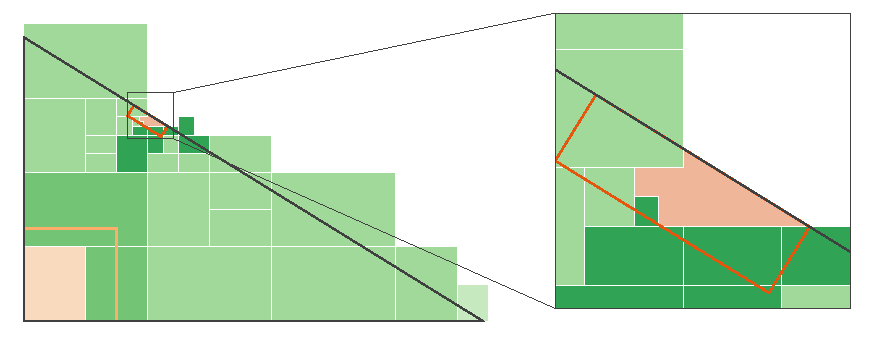
\includegraphics[width=\linewidth]{figures/local-tiling}
\caption{The viewing parameters of the covers around aligned configurations, $s\in[0,2/3]$ horizontally and $t\in[0,2/5]$ vertically, with the viewing triangle outlined: the 30 rows of \cref{tab:local-covers} before enlargement, shaded by their radius (\fc{TileLight}{lightest $1/20$}, then \fc{Sheared}{$1/50$}, \fc{Local}{$1/80$ and $1/96$}, \fc{TileDark}{darkest $1/200$}); \fc{Square}{the square cover's views $[0,1/8]^2$ (light orange)}; and \fc{Pentagon}{the pentagon cover's parallelogram $|\eta|\le1/32$, $-1/32\le\xi\le0$ (red-orange)}. The square and pentagon covers, each a single region, are lightly tinted beneath the rows, which overlap them, and outlined on top. Right: the neighbourhood of the pentagon's viewing parameters, enlarged, where the rows approach the edge-on line in steps.}
\label{fig:local-tiling}
\end{figure}

\begin{table}[ht]
\centering\footnotesize
\setlength{\tabcolsep}{2.2pt}
\begin{tabular}{lllllrrr}
  \toprule
  Cover & Kind & Base; offset & Parameters & Zooms & Cells & Domain & Handed\\
  \midrule
  square & point & $(s,t)$, $\Sigma={[0,1]}^2$; $\mathbf r$ & $\mu_{\max}=\delta_{\max}=\frac18$, $\rho_0=1$ & 18 & 877 & 95 & --\\
  pentagon & point & $(\eta,\xi)$, $\Sigma=[-1,1]{\times}[-1,0]$; $\mathbf r$ & $\mu_{\max}=\frac1{32}$, $\delta_{\max}=\frac1{16}$, $\rho_0=2$ & 24 & 6{,}173 & 0 & --\\
  arc$\pm$ & tube & $e\in[\frac3{64},\frac3{16}]$; $(\frac v2,\theta,\zeta_1,\zeta_3)$ & $\delta_{\max}=\frac1{32}$ & 7 & 343, 288 & 32, 72 & --\\
  endpoint$\pm$ & point & $e-e_*$; $(\frac v2,\theta,\zeta_1,\zeta_3)$ & $\mu_{\max}=\frac1{16},\frac1{32}$, $\delta_{\max}=\frac1{32}$, $\rho_0=1$ & 21 & 305, 246 & 10, 50 & --\\
  crossing$\pm$ & point & $e$; $(\frac{4v}5,\theta,\zeta_1,\zeta_3)$ & $\mu_{\max}=\delta_{\max}=\frac1{16}$, $\rho_0=\frac54$, $\rho_0'=\frac14$ & 28 & 1{,}431, 687 & 31, 160 & 34, 14\\
  \bottomrule
\end{tabular}
\caption{The eight covers of the Exotic component. The offset box is
$\Phi={[-1,1]}^3$ for the square and pentagon and $\Phi=[0,1]\times{[-1,1]}^3$
along the arcs; the pairs are for $\sigma=1$ and $\sigma=-1$, and the
endpoint's two base radii are for $e<e_*$ and $e>e_*$. \emph{Zooms} counts
the zooms of one cover, including the seven sheared zooms of each crossing
cover; \emph{Cells} counts the terminal cells with a witness, and
\emph{Domain} those among them whose witness is an inequality of $D$ (the
fold for $g=k$ at the square, the tie inequality along the arcs).
\emph{Handed} counts the cells handed over by \cref{lem:hand-over}.}
\label{tab:exotic-covers}
\end{table}
